\documentclass{beamer}

% Imported Packages
\usepackage[utf8]{inputenc}
\usepackage{xcolor}
\usepackage{amsmath, amssymb}

% Theme
\usetheme[white, compactlogo]{Wisconsin}
\setbeamertemplate{caption}[numbered]
\renewcommand{\vec}[1]{\mathbf{#1}}

%This block of code defines the information to appear in the
%Title page
\title{QT-Opt: Scalable Deep Reinforcement Learning for Vision-Based Robotic Manipulation}
\subtitle{arXiv:1806.10293, Kalashnikov et al, 2018.}
\author{\textit{Sumamrized by} Hyecheol (Jerry) Jang}
\institute{
  Department of Computer Sciences\\
  University of Wisconsin–Madison
}
\date{RL Paper Study, Jun. 29. 2020}
%End of title page configuration block
%------------------------------------------------------------


%------------------------------------------------------------
%The next block of commands puts the table of contents at the 
%beginning of each section and highlights the current section:

\AtBeginSection[]
{
  \begin{frame}
    \frametitle{Table of Contents}
    \tableofcontents[currentsection]
  \end{frame}
}
%------------------------------------------------------------


%---------------------------------------------------------
%This block defines the existing sections
\newcommand{\firstSec}{Motivation}
\newcommand{\secondSec}{Goal}
\newcommand{\thirdSec}{Overview of Model Architecture}
\newcommand{\forthSec}{QT-Opt}
\newcommand{\fifthSec}{Environment Settings}
\newcommand{\sixthSec}{Experiments}
\newcommand{\seventhSec}{Discussions}
\newcommand{\refSec}{Bibliography}
%---------------------------------------------------------


\begin{document}
  %The next statement creates the title page.
  \frame{\titlepage}

  % Section 1, Motivation
  \section{\firstSec}
    \begin{frame}
      \frametitle{\firstSec : Why Robotics + Reinforcement Learning}
      \begin{itemize}
        \item Usually, Robots are good at \textbf{repetitive tasks} (e.g. Assembly Line)
              \pause
        \item Want to make Robots that \textbf{identifies surroundings} and \textbf{behave accordingly},
              but it is difficult
              \pause
        \begin{itemize}
          \item \textbf{Deep Learning}\\
                Provide ability to handling real-world scenarios
          \item \textbf{Reinforcement Learning}\\
                Provide ability to make decision in long-term,
                using previous experiences in complex and robust scenarios
        \end{itemize}
        \pause
        \item Combining two techniques
        \begin{itemize}
          \item Able to learn policy continuously from their experience
          \item No need for manual engineering, use data they collects
        \end{itemize}
      \end{itemize}
    \end{frame}

    \begin{frame}
      \frametitle{\firstSec : Difficulites of Using RL in Robotics}
      \begin{itemize}
        \item Varience in \textbf{visual and physical property of objects}
        \pause
        \begin{itemize}
          \item Hardness of object (Soft or Hard)
          \item Surface Characteristics (Slippery, Sticky, \ldots)
          \item Color Variation
          \item Shape Variation
          \item \ldots
        \end{itemize}
        \pause
        \item \textbf{Noise} of sensors
      \end{itemize}
      \pause
      \begin{itemize}
        \setlength{\itemindent}{.3in}
        \item[$\Rightarrow$] Still hard to handle though we have sufficiently large training set
        \begin{itemize}
          \setlength{\itemindent}{0.3in}
          \item[$\Rightarrow$] Collecting those training set is expensive (real experiments) 
        \end{itemize}
      \end{itemize}
    \end{frame}

    \begin{frame}
      \frametitle{\firstSec : Previous Works}
      \begin{itemize}
        \item Focused on learning narrow, individual tasks
        \begin{itemize}
          \item hitting a ball
          \item opening door
          \item throwing objects
          \item \ldots
        \end{itemize}
        \pause
      \end{itemize}
      \begin{itemize}
        \setlength{\itemindent}{.3in}
        \item[$\Rightarrow$] Use \textbf{Grasping} to achieve \textit{generalization}
      \end{itemize}
      \pause
      \begin{itemize}
        \item Approached the grasping task as predicting a \textit{grasp pose}
        \begin{enumerate}
          \item Observe the scene (\textit{Normally, using a depth camera})
          \item Choose best location to grasp
          \item Reach the location (open-loop setting)
        \end{enumerate}
        \pause
        \begin{itemize}
          \item Different with how humans and animals behave
          \item Grasp is a \textbf{dynamical process} that sence and control at each stage
        \end{itemize}
      \end{itemize}
      \pause
      \begin{itemize}
        \setlength{\itemindent}{.3in}
        \item[$\Rightarrow$] \textbf{Where this researches start!!}
      \end{itemize}
    \end{frame}
  % End of Section 1


  % Section 2: Goal
  \section{\secondSec}
  \begin{frame}
    \frametitle{\secondSec}
    \centering
    \Large{Use Reinforcement Learning with Deep Neural Network\\
           to \textbf{perform pre-grasp manipulation}, \\
           \textbf{response to dynamic disturbances}, \\
           and \textbf{learn grasping in a generic framework} \\
           that makes minimal assumptions about the task}
  \end{frame}

  \begin{frame}
    \frametitle{\secondSec : Constraint/Condition + Literature Review}
    \begin{itemize}
      \item \textbf{Closed-loop condition} (With feedback, \textit{\scriptsize{Morrison, et al.}})
      \begin{itemize}
        \item For the other papers work on closed-loop grasping, they deals with servoing problems.
        \item This paper focuses on making generalized RL algorithm
        \item In practice, it makes Kalashnikov et al.'s method (this method)
              to autonomously acquire complicated grasping strategy
      \end{itemize}
      \pause
      \item \textbf{Self-supervised} learning task
      \begin{itemize}
        \item Compare to prevoius work(by Zeng et al.), Kalashnikov et al. utilize more general action space
        \item Actions consist of end-effector \textbf{Cartesian motion} and \textbf{gripper opening/closing}
      \end{itemize}
      \pause
      \item Observation comes from \textbf{a single RGB camera} over the sholder
      \begin{itemize}
        \item Many current grasping system utilizes depth sensing
        \item Using wrist-mounted cameras
      \end{itemize}
    \end{itemize}
  \end{frame}
  % End of Section 2


  % Section 3: Overview of Model Architecture
  \section{\thirdSec}
    \begin{frame}
      \frametitle{\thirdSec : MDP}
      \begin{itemize}
        \item General Formulation of Robotic Manipulation: \\
              Based on \textbf{Markov Decision Process (MDP)}
        \begin{itemize}
          \item partially observed formulation (POMDP) is more general.
          \item However, assuming current observation contains all necessary information for this task,
                it is sufficient to use MDP.
        \end{itemize}
        \pause
        \item MDP have a \textbf{general and powerful formalism} for decision making problems. \\
              However, it is \textbf{hard to train}
        \pause
        \item For each step of MDP:
        \begin{enumerate}
          \item Observes Image from robot's camera (see Fig. \ref{fig:WorkspaceOverview})
          \item choose a gripper command, Reward:
          \begin{itemize}
            \item failed grasp: reward of 0
            \item successful grasp: reward of 1 \\
                  Defined \textit{success} when the robot holds the object above a certain height
          \end{itemize}
        \end{enumerate}
      \end{itemize}
    \end{frame}

    \begin{frame}
      \frametitle{\thirdSec: MDP}
      \begin{figure}
        \begin{columns}
          \column{.4\linewidth}
            \centering
            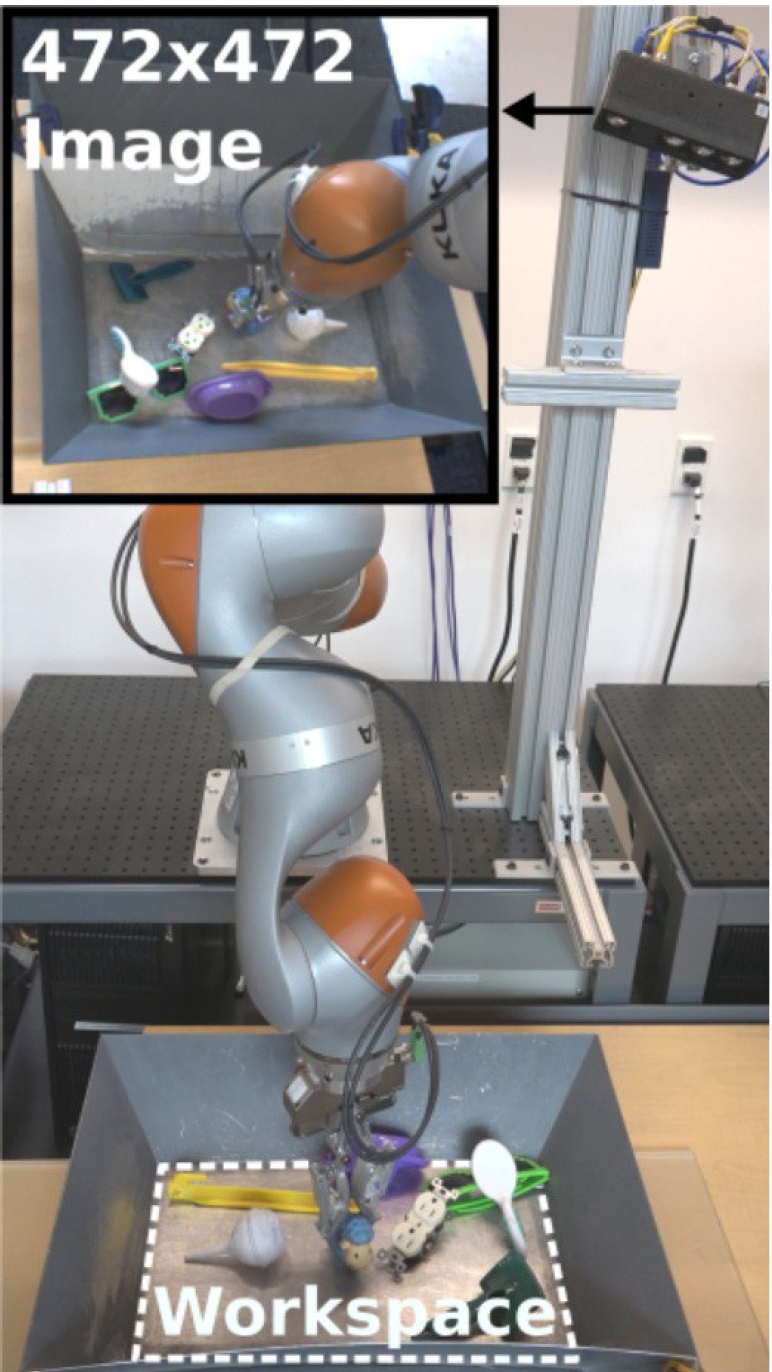
\includegraphics[height=0.82\textheight]{Images/WorkspaceOverview.png}
          \column{.6\linewidth}
            \caption{Configuration of robot cell, with a sample observation image on top-right box}
            \label{fig:WorkspaceOverview}
        \end{columns}
      \end{figure}
    \end{frame}

    \begin{frame}
      \frametitle{\thirdSec: Algorithm Selection}
      \begin{itemize}
        \item Usually, Generalization needs diverse data
        \begin{itemize}
          \item However, recollecting experience on numerous objects after every policy update is impractical
          \item Reason for \textbf{not using on-policy algorithm}
        \end{itemize}
        \pause
        \item Using \textbf{scalable off-policy algorithm} based on Q-learning
        \begin{itemize}
          \item actor-critic algorithm are popular for handling continuous actions
          \item However, Kalashnikov et al. found \textbf{scalable and more stable ways} to train only Q-function
        \end{itemize}
        \pause
        \item Large Dataset and Network (See Fig. \ref{fig:ModelStructure})
        \begin{itemize}
          \item Kalashnikov et al. devised \textbf{distributed} training system (with 7 robots)
          \item \textbf{Asynchronously update} target values, collect \textbf{on-policy data}, \\
                reloads \textbf{off-policy data} from previous experiences, \\ 
                and train network on both data stream.
        \end{itemize}
      \end{itemize}
    \end{frame}

    \begin{frame}
      \frametitle{\thirdSec : Algorithm Selection}
      \begin{figure}
        \centering
        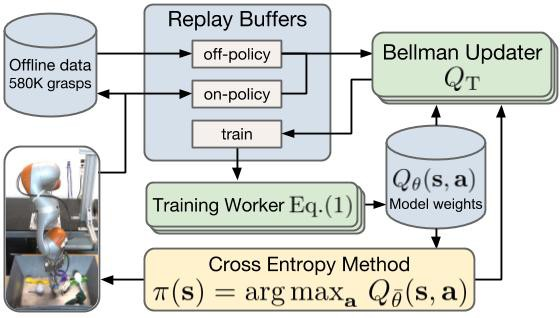
\includegraphics[]{Images/ModelStructure.jpg}
        \caption{Distributed Reinforcement Learning infrastructure for QT-Opt.}
        \label{fig:ModelStructure}
      \end{figure}
    \end{frame}

    \begin{frame}
      \frametitle{Optional: On-policy vs Off-policy \scriptsize{\textit{Poole et al.}}}
      \begin{itemize}
        \item \textbf{On-policy Learning} learns the value of the policy being \textbf{carried out by the agent}, including the exploration steps. \\
              e.g. SARSA(State-Action-Reward-State-Action) (See Fig. \ref{fig:SARSAAlgorithm})
        \pause
        \item \textbf{Off-policy Learning} learns the value of the optimal policy \textbf{independently of the agent's action} \\
              e.g. Q-Learning (See Fig. \ref{fig:QLearningAlgorithm})
      \end{itemize}
    \end{frame}

    \begin{frame}
      \frametitle{Optional: On-policy vs Off-policy \scriptsize{\textit{Poole et al.}}}
      \begin{columns}[b]
        \column{.5\linewidth}
          \centering
          \begin{figure}
            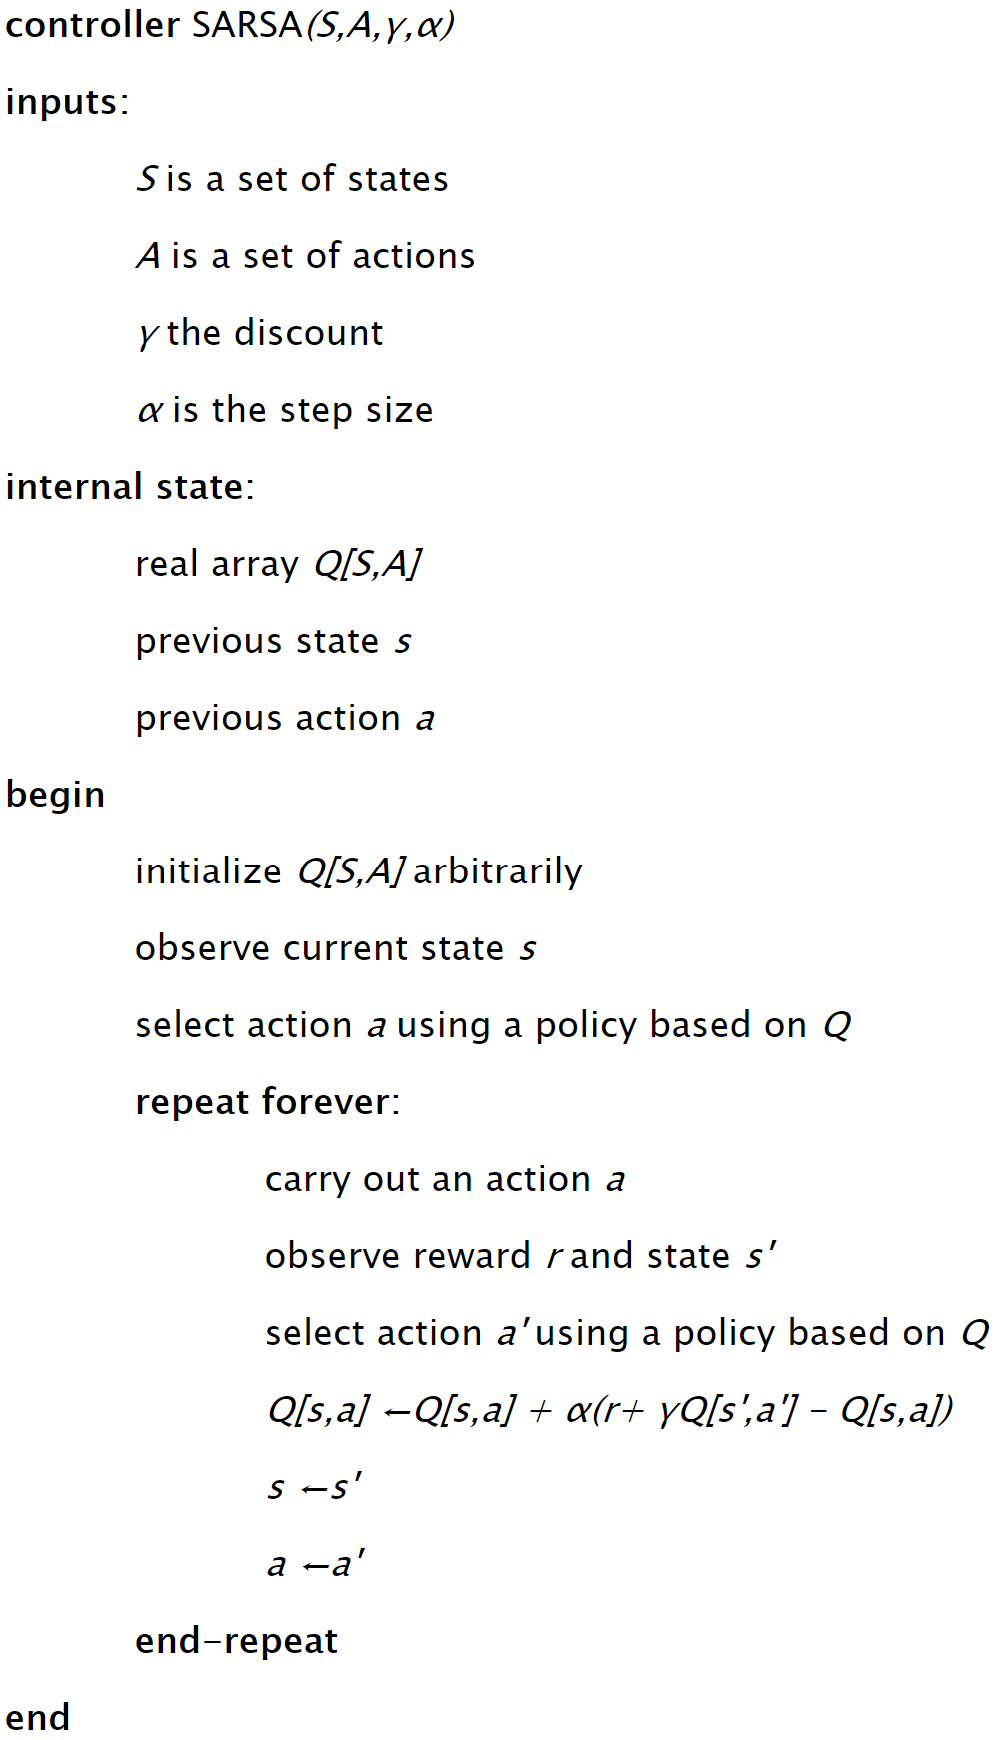
\includegraphics[height=.75\textheight]{Images/SARSA.png}
            \caption{SARSA Algorithm}
            \label{fig:SARSAAlgorithm}
          \end{figure}
         \column{.5\linewidth}
           \centering
           \begin{figure}
             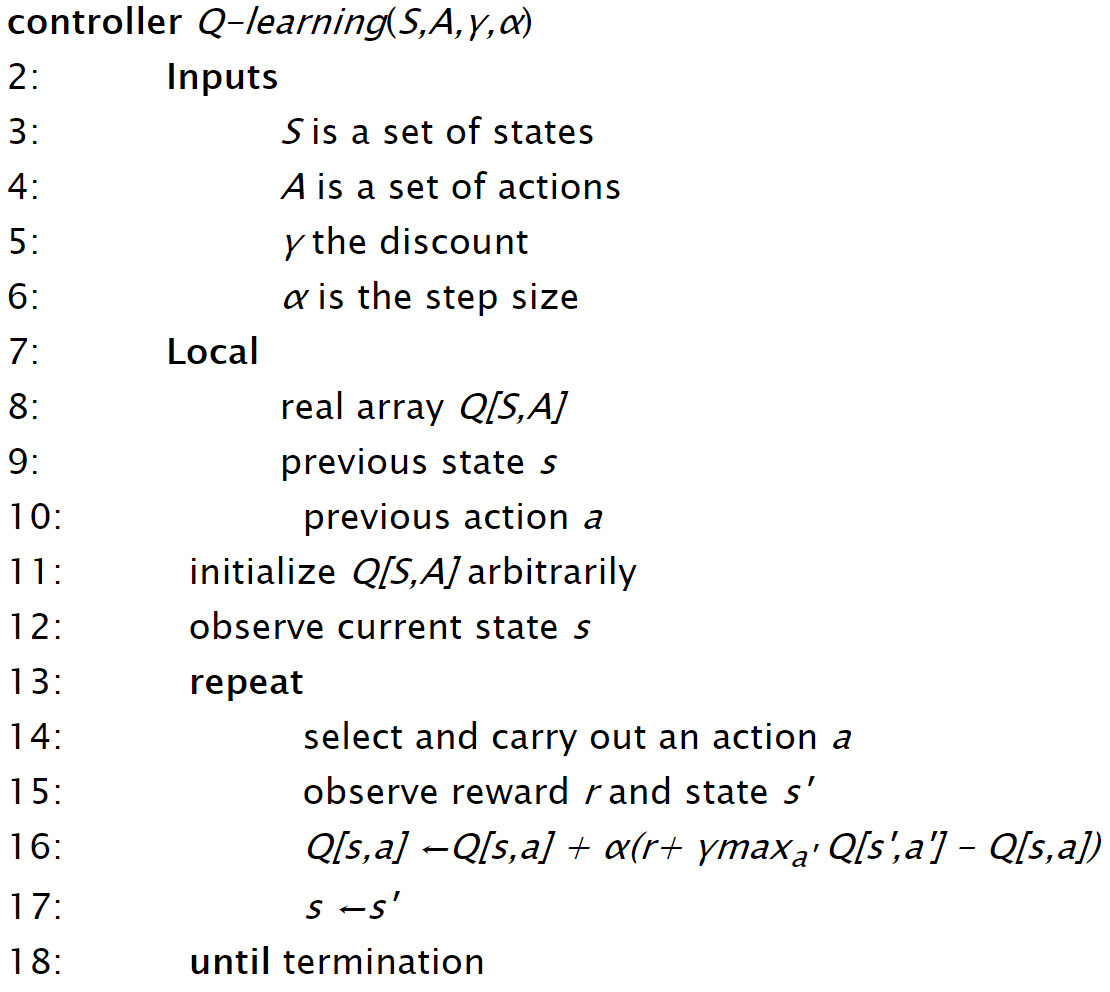
\includegraphics[width=.9\linewidth]{Images/Q-Learning.png}
             \caption{Q-Learning Algorithm}
             \label{fig:QLearningAlgorithm}
           \end{figure}
      \end{columns}
    \end{frame}
  % End of Section 3


  % Section 4: QT-Opt
  \section{\forthSec}
    \begin{frame}
      \frametitle{\forthSec}
      \begin{itemize}
        \item \Large{Continuous action version of Q-Learning}
        \begin{itemize}
          \item For \textbf{scalable} learning and optimized for \textbf{stability}
          \item To handle \textbf{large amount of off-policy image data} for complex tasks
        \end{itemize}
      \end{itemize}
    \end{frame}

    \begin{frame}
      \frametitle{\forthSec: Revisit Q-Learning}
      \begin{itemize}
        \item \textbf{state}: $\vec{s} \in \mathcal{S}$ (\textit{Image Observations})
        \item \textbf{action}: $\vec{a} \in \mathcal{A}$ (\textit{Robot Arm Motions and Gripper commands})
        \item at \textbf{each time step} $t$
        \begin{enumerate}
          \item Choose an action
          \item transition to new state
          \item receive reward $\gamma(\vec{s}_t, \vec{a}_t)$
        \end{enumerate}
      \end{itemize}
    \end{frame}

    \begin{frame}
      \frametitle{\forthSec: Revisit Q-Learning}
      \begin{itemize}
        \item Need to solve for Optimal Q-function: Minimize Bellman Error \\
              \begin{equation*}
                \mathcal{E}(\theta) = \mathbb{E}_{(\vec{s}, \vec{a}, \vec{s'}) \sim p(\vec{s}, \vec{a}, \vec{s'})}[\mathcal{D}(\mathcal{Q}_{\theta}(\vec{s}, \vec{a}),\mathcal{Q}_{\mathcal{T}}(\vec{s}, \vec{a}, \vec{s'}))]
              \end{equation*}
              Where $\mathcal{Q}_{\mathcal{T}}(\vec{s}, \vec{a}, \vec{s'}) = r(\vec{s}, \vec{a}) + \gamma V(\vec{s'})$ (\textit{target value})
        \item $\mathcal{D}$: divergence metric (squared difference for Q-Learning)
        \linebreak
        \item Expectation is taken under the distribution over all previously observed transition
      \end{itemize}
    \end{frame}

    \begin{frame}
      \frametitle{\forthSec: Q-Learning Implementation}
      \begin{itemize}
        \item Use \textbf{two target network} to improve stability
        \begin{itemize}
          \item Maintaining two lagged version of the parameter vector $\theta, \bar{\theta_1}, \bar{\theta_2}$
          \item $\bar{\theta_1}$: exponential moving averaged version of $\theta$, \\ 
                averaging constant: 0.9999
          \item $\bar{\theta_2}$: lagged version of $\bar{\theta_1}$, \\
                lagged by 6000 gradient steps
        \end{itemize}
        \pause
        \item Compute target value by $V(\vec{s'}) = \min_{i = 1, 2}\mathcal{Q}_{\bar{\theta_i}}(\vec{s'}, arg\max_{\vec{a'}}\mathcal{Q}_{\bar{\theta_1}}(\vec{s'}, \vec{a'}))$
        \pause
        \item the policy is recovered by $\pi(\vec{s}) = arg\max_{\vec{a}}\mathcal{Q}_{\bar{\theta_1}}(\vec{s}, \vec{a})$
        \pause
        \item After collects samples from environment interaction, then perform off-policy training on all samples collected
        \begin{itemize}
          \item Problem: Large-scale learning (Technically Difficult)
          \item Solution: Use \textbf{Parallel Asynchronous} version \\
                (which leads ability to scale up the process)
        \end{itemize}
      \end{itemize}
    \end{frame}

    \begin{frame}
      \frametitle{\forthSec: Problem of Q-Learning}
      \begin{itemize}
        \item Difficult to deal with continuous actions, \footnotesize{e.g. continuous gripper motion}
        \pause
        \item \normalsize{\textit{Previous Solutions:}}
        \begin{itemize}
          \item using a second network that "amortize" the maximization
          \item constraining the Q-function to be convex in $\vec{a}$, so that makes the function to easily find maximum ananlytically
        \end{itemize}
        \pause
        \item problem of previous solutions
        \begin{itemize}
          \item Unstable: problematic for large-scale RL tasks where running hyperparameter sweeps is very expensive
          \item Action-convex value functions are poor fit for complex manipulation tasks \\
        \end{itemize}
      \end{itemize}
    \end{frame}

    \begin{frame}
      \frametitle{\forthSec : Stable Continuous-Action Q-Learning}
      \begin{itemize}
        \item To \textbf{maintain the generality of non-convex Q-function} \\ 
              while \textbf{not using a second maximizer network}
        \item the Bellman equation is evaluated with stocastic optimization
        \begin{itemize}
          \item handles non-convex and multimodal optimization landscapes
          \linebreak
        \end{itemize}
        \pause
        \item QT-Opt
        \begin{itemize}
          \item $\pi_{\bar{\theta_1}}(\vec{s})$ is evaluaed by running stochastic optimization over $\vec{a}$, \\
                using $\mathcal{Q}_{\bar{\theta_1}}(\vec{s}, \vec{a})$ as the objective value
          \pause
          \item Use Cross-Entropy Method
          \begin{enumerate}
            \item samples a batch of $N$ at each iteration
            \item fits a Gaussian distribution to the best $M < N$ samples
            \item Samples next batch of $N$ from the Gaussian
            \pause
          \end{enumerate}          
          \begin{itemize}
            \item easy to parallelize
            \item moderately robust to local optima
          \end{itemize}
        \end{itemize}
      \end{itemize}
    \end{frame}

    \begin{frame}
      \frametitle{\forthSec : Distributed Asynchronous QT-Opt}
      \begin{itemize}
        \item Requires large amount of diverse data to generalize over new scenes and objects for the image-based policy
        \linebreak
        \pause
        \item Needs of Distributed System (See Fig. \ref{fig:ModelStructure})
        \pause
        \begin{enumerate}
          \item Replay buffer stores both \textbf{off-line data} (from disk) and \\ 
                on-going experiments' data (\textbf{on-line data})
          \pause
          \item Data in buffer labeled with target Q-value using a set of 1000 \\
                "bellman updater" jobs
          \pause
          \item Store the labeled sample in the training buffer
          \begin{itemize}
            \item Some samples in the training buffer are \textbf{labeled with lagged version} \\ 
                  of the Q-network
          \end{itemize}
          \pause
          \item Training workers pull the labeled sample from the training buffer \textbf{randomly} to update the Q-function
          \begin{itemize}
            \item each training workers compute gradient that sent to \\ 
                  parameter server asynchronously
          \end{itemize}
        \end{enumerate}
        \pause
        \begin{itemize}
          \item Empirically, it requires up to \textbf{15M gradient steps} \\
                to train effective Q-function due to \textbf{complexity of the task} \\ 
                and \textbf{the size of dataset and model}
        \end{itemize}
      \end{itemize}
    \end{frame}
  % End of Section 4


  % Section 5: Environment Settings
  \section{\fifthSec}
    \begin{frame}
      \frametitle{\fifthSec : Overview}
      \begin{itemize}
        \item Policy
        \begin{itemize}
          \item locate object
          \item position for grasping (pre-grasping manipulation, if needed)
          \item pick up (regrasping, if needed)
          \item Pull up the object
          \item signal thermination
        \end{itemize}
        \pause
        \item Reward
        \begin{itemize}
          \item only indicates whether or not an object was successfully picked up
        \end{itemize}
        \pause
        \item End-to-End approach of grasping!!
        \begin{itemize}
          \item no prior knowledge about object, physics, or motion planning
          \item model itself autonomously extract the knowledges from data
        \end{itemize}
      \end{itemize}
    \end{frame}

    \begin{frame}
      \frametitle{\fifthSec : MDP for grapsing}
      \begin{itemize}
        \item state observation $\vec{s} \in \mathcal{S}$ includes:
        \begin{itemize}
          \item robot's current camera observation (RGB image, res: 472 $\times$ 472) \\
                from over-the-sholder single-lens camera
          \item current status of gripper (binary)
          \item vertical position of the gripper relative to the floor
        \end{itemize}
        \pause
        \item action $\vec{a} = (\vec{t}, \vec{r}, g_{open}, g_{close}, e) \in \mathcal{A}$ includes:
        \begin{itemize}
          \item vector in Cartesian space $\vec{t} \in \mathbb{R}^3$ \\ 
                (desired change in the gripper position)
          \item change in azimuthal angle via sine-cosine encoding, $\vec{r} \in \mathbb{R}^2$
          \item binary gripper open and close command, $g_{open}, g_{close}$
          \item termination command, $e$
        \end{itemize}
      \end{itemize}
    \end{frame}

    \begin{frame}
      \frametitle{\fifthSec : Reward Function}
      \begin{itemize}
        \item 1: if gripper carries the object up above certain height \\ 
              at the end of the episode
        \item 0: otherwise
        \pause
        \item penalty (-0.05): for all time steps prior to termination
        \begin{itemize}
          \item emits termination action
          \item exceed the maximum number of time steps(20)
          \linebreak
        \end{itemize}
        \pause
        \item delayed and sparse reward function is challenging, \\
              but more practical for automated self-supervision
      \end{itemize}
    \end{frame}

    \begin{frame}
      \frametitle{\fifthSec : Q-function}
      \begin{figure}
        \centering
        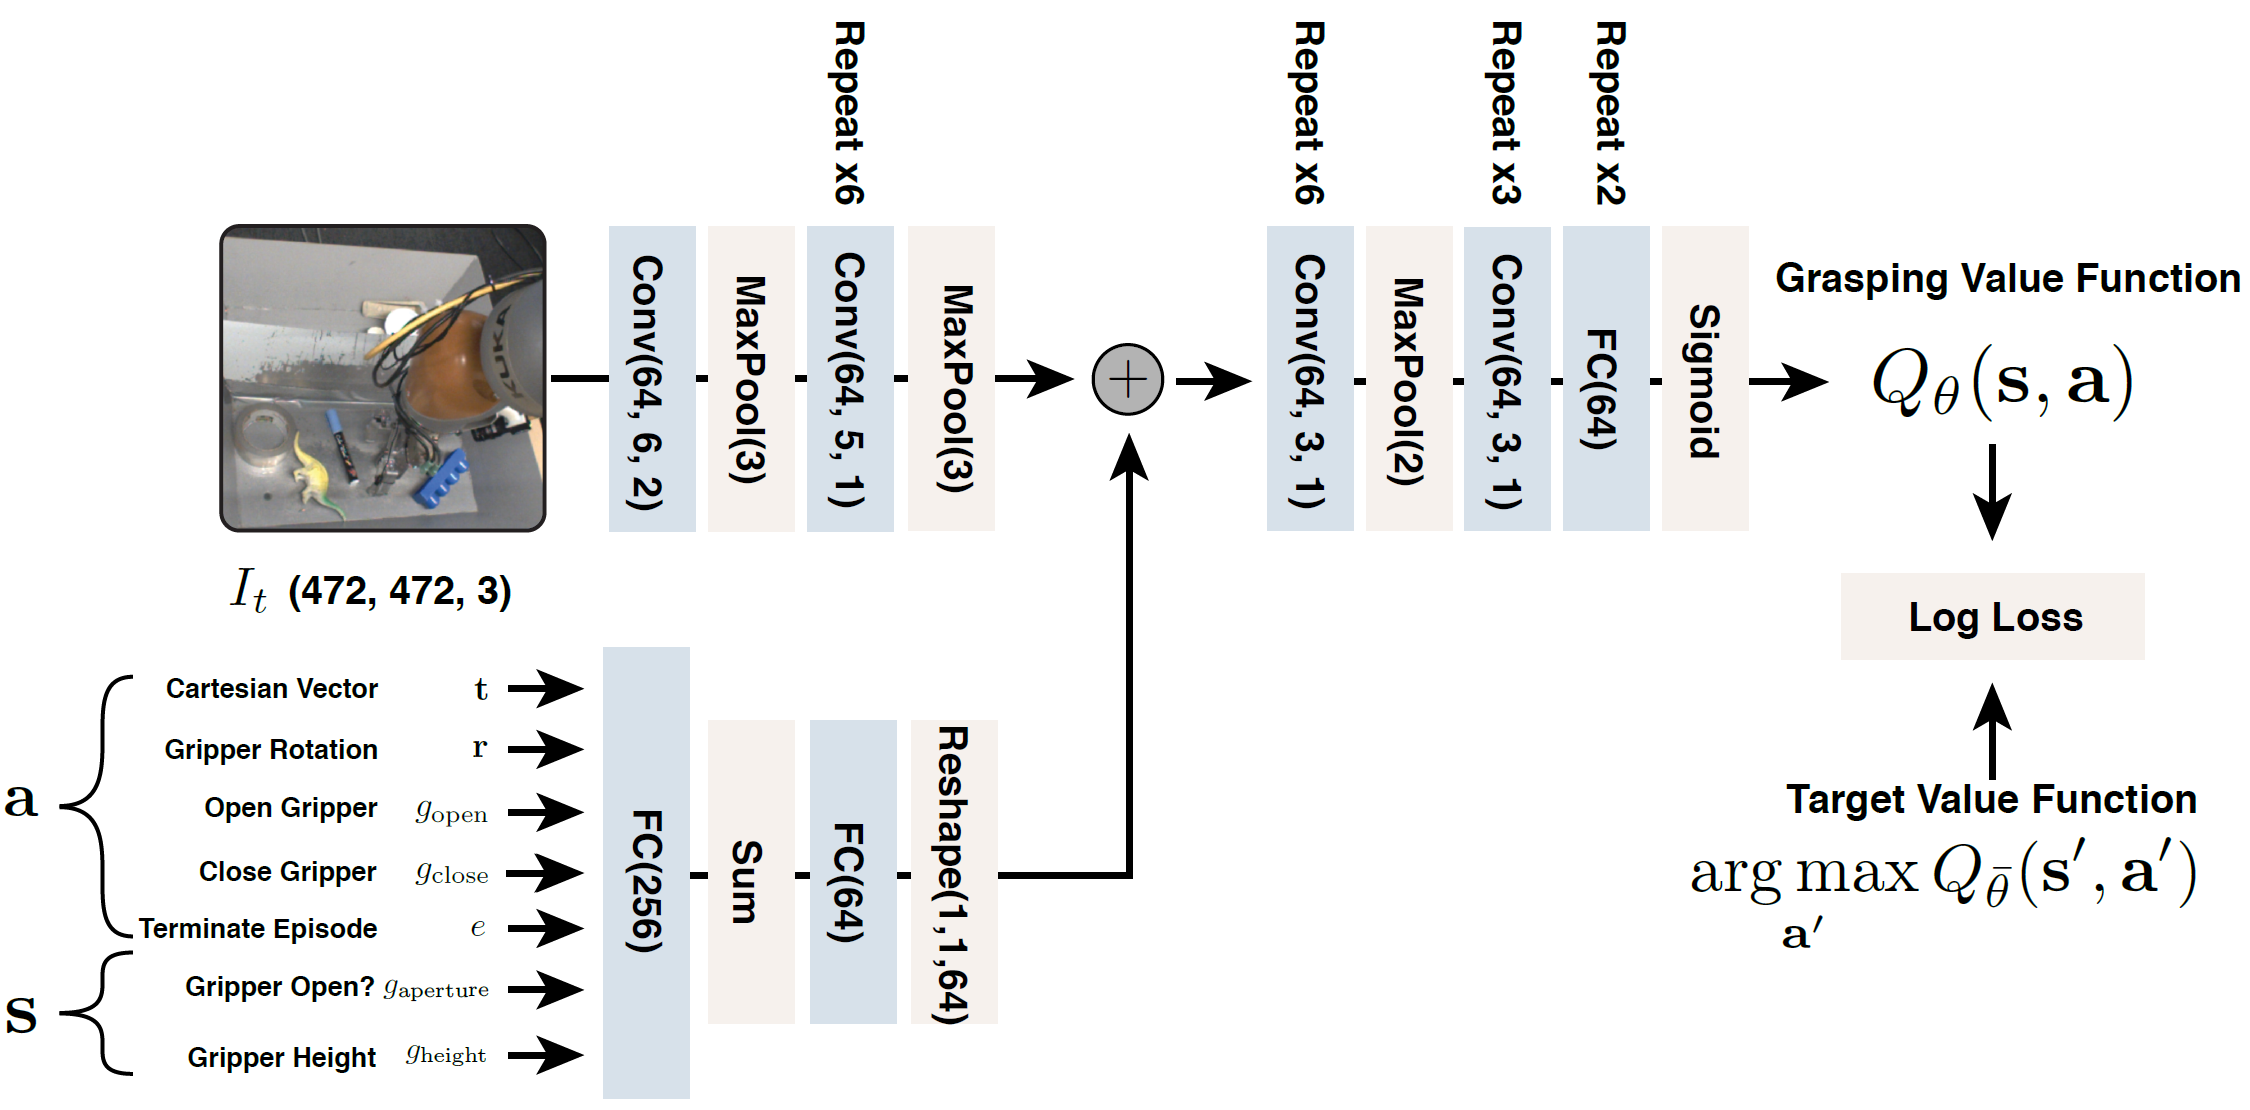
\includegraphics[width = \linewidth]{Images/QFunctionNetwork.png}
        \caption{Neural Network Architecture for Q-Fuction. \linebreak
                 It has total of 1.2M parameters. The image is processed with convolution filters,
                 and the other inputs are processed by fully connected layer, then concatenated with the image}
        \label{fig:QFunctionNetwork}
      \end{figure}
    \end{frame}

    \begin{frame}
      \frametitle{\fifthSec : Data Collection}
      \begin{itemize}
        \item Need to collect data on sufficiently large and diverse set of objects
        \item Use multiple robots and multiple experiments to collect such data
        \begin{itemize}
          \item Took four months, 800 Robot hrs
          \item Collected during multiple separated experiments, \\
                and each experiment reused the data from the previous one
          \linebreak
        \end{itemize}
        \pause
        \item Initialize policy
        \begin{itemize}
          \item Used weak scripted exploration policy to bootstrap data collection
          \item Still random, but biased toward reasonable grapsing
          \item Success Rate: Around 15-30\%
          \item Switching to QT-Opt once it reach 50\% of success rate
          \linebreak
        \end{itemize}
        \pause
        \item Other Conditions
        \begin{itemize}
          \item Using seven LBR IIWA robots
          \item with 4-10 objects per robots
          \item objects were replaced every 4 hours during business hours
          \item Use different objects during test
        \end{itemize}
      \end{itemize}
    \end{frame}
  % End of Section 5


  % Section 6: Experiments
  \section{\sixthSec}
    \begin{frame}
      \frametitle{\sixthSec}
      \begin{enumerate}
        \item Performance on unseen object (quantitative)
        \item Performance comparision with other self-supervised grasping system (quantitative)
        \item Manipulation strategies which carried out meaningful pre-grasp manipulation (quality)
      \end{enumerate}
    \end{frame}

    \begin{frame}
      \frametitle{\sixthSec : Quantitative Analysis}
      \begin{itemize}
        \item Used two evaluation protocol
        \begin{itemize}
          \item Each robots make 102 grasp attemps on test objects.
          \begin{itemize}
            \item grasp attemps last for up to 20 times steps
            \item any grasped objects returned back to the bin
            \item Experimently, the robot made grasp attemps on a various objects, \\
                  not picking one objects
            \item Might have confounding effects
          \end{itemize}
          \pause
          \item bin emptying
          \begin{itemize}
            \item single robot unload a bin with 28 test objects, using 30 grasp attemps
            \item Repeated for five times
            \item Success rate is reported over the first 10, 20, and 30 grasp attemps
          \end{itemize}
        \end{itemize}
      \end{itemize}
    \end{frame}

    \begin{frame}
      \frametitle{\sixthSec: Quantitative Analysis (Result)}
      \begin{figure}
        \centering
        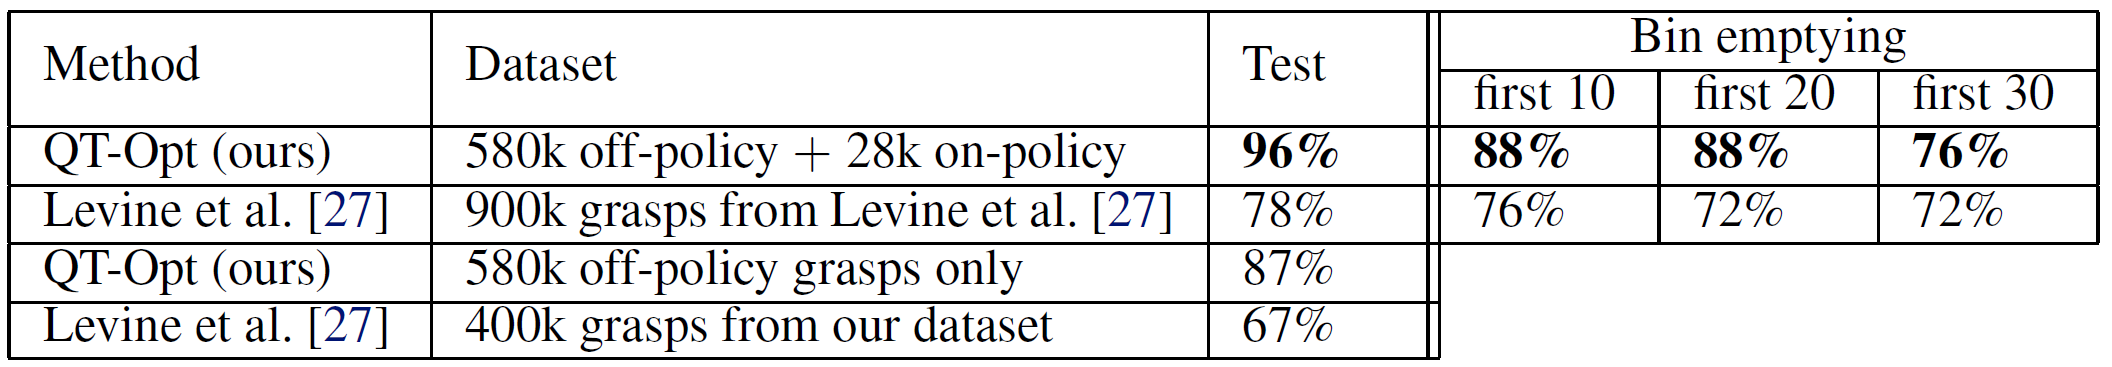
\includegraphics[width = \linewidth]{Images/QuantitativeAnalysisResult.png}
        \caption{Result of Quantitative Analysis Result. \linebreak
                 Left half indicates the result of re-deposit grasping tasks, the right half indicates the results of bin emptying experiments}
        \label{fig:QuantitativeAnalysisResult}
      \end{figure}
    \end{frame}

    \begin{frame}
      \frametitle{\sixthSec: Quantitative Analysis (Result)}
      (See Fig. \ref{fig:QuantitativeAnalysisResult})
      \begin{itemize}
        \item Usage of on-policy training
        \begin{itemize}
          \item on-policy joint finetuning provides better Performance
          \item Kalashnikov et al. analyzed that on-policy helps the model to remove "hard negatives"
        \end{itemize}
        \pause
        \item Bin emptying
        \begin{itemize}
          \item successfully empty all objects within 30 grasps for 2/5 trials (Kalashnikov et al.)
          \item Previous method (Levine et al.) successfully empty for 1/5 trials
          \item lower success rate for 30 grasp due to the algorithm tend to grasp easy one first
        \end{itemize}
      \end{itemize}
    \end{frame}

    \begin{frame}
      \frametitle{\sixthSec: Quantitative Analysis (Result)}
      (See Fig. \ref{fig:QuantitativeAnalysisResult})
      \begin{itemize}
        \item Compare with Levine et al.
        \begin{itemize}
          \item greedly optimized for grasp success at the next grasp
          \item does not control the opening and closing of gripper
          \item does not explain about pregrasp manipulation
          \pause
          \item action representation is different, making the format of dataset different
          \pause
          \item tested on both Levine et al.'s data format and this article's format
          \item either way, it is worse than Kalashnikov et al's work
        \end{itemize}
      \end{itemize}
    \end{frame}

    \begin{frame}
      \frametitle{\sixthSec : Qualitative Analysis}
      \centering
      Video: \url{https://sites.google.com/view/qtopt}
    \end{frame}

    \begin{frame}
      \frametitle{\sixthSec : Qualitative Analysis (Explaination)}
      \begin{itemize}
        \item Singulation and pregrasp manipulation
        \begin{itemize}
          \item Change position of object to make them easier to grasp
        \end{itemize}
        \pause
        \item Regrasping
        \begin{itemize}
          \item open and close the gripper at any time
          \item detect failed or unstable grasp earlier \\
                so that let the robots to grisp more securely
        \end{itemize}
        \pause
        \item Handling disturbance and Dynamic objects
        \begin{itemize}
          \item grasp object that moving dynamically (e.g. balls)
          \item though the sequence intentionally disturbed, \\ 
                it still able to grasp the object
        \end{itemize}
        \pause
        \item Grapsing in clutter
        \begin{itemize}
          \item Note that there exists upto 10 objects during training time
          \item The policy still able to grasp object in dense clutter
          \pause
          \item Some failure
          \begin{itemize}
            \item prone to regrasp repeatedly
            \item often produce successful graps, but time consuming
          \end{itemize}
        \end{itemize}
      \end{itemize}
    \end{frame}
  % End of Section 6


  % Section 7: Discussions
  \section{\seventhSec}
    \begin{frame}
      \frametitle{\seventhSec}
      \begin{itemize}
        \item Scalable robotics RL with raw sensory input, with QT-Opt, \\ 
              a distributed optimization framework
        \item combination of off-policy and on-policy training
        \item The model able to learn sophisticated behaviors (singulation, pregrasp manipulation, regrasping, and dynamic response toward disturbance)
        \item All experience is collected autonomously
        \item Amount of required data is lower than the benchmark
      \end{itemize}
    \end{frame}
  % End of Section 7


  % Endings: Bibliography
  \section{\refSec}
    \begin{frame}[allowframebreaks]
      \frametitle{\refSec}
      \begin{itemize}
        \item \textbf{Kalashnikov, Dmitry, et al. QT-Opt: Scalable Deep Reinforcement Learning for Vision-Based Robotic Manipulation. 28 Nov. 2018, arxiv.org/abs/1806.10293.}
        \item Irpan, Alex, and Peter Pastor. Scalable Deep Reinforcement Learning for Robotic Manipulation. 28 June 2018, ai.googleblog.com/2018/06/scalable-deep-reinforcement-learning.html.
        \item Morrison, Douglas, et al. “Closing the Loop for Robotic Grasping: A Real-Time, Generative Grasp Synthesis Approach.” Robotics: Science and Systems XIV, 2018, doi:10.15607/rss.2018.xiv.021.
        \item Poole, David Lynton, and Alan K. Mackworth. Artificial Intelligence: Foundations of Computational Agents. Cmabridge University Press, 2018.
      \end{itemize}
    \end{frame}
  % End of Reference Lists

\end{document}
